\documentclass[11pt]{article}

\usepackage{amssymb}
\usepackage{amsmath}
\usepackage{amsthm}
\usepackage{indentfirst}
\usepackage{graphicx}

\title{MA 590 Homework 2}
\author{Dane Johnson}

\begin{document}
\maketitle

\section*{Problem 1}

Consider a downward propagating seismic wavefront generated by a source on the surface where the observed travel time in seconds, $t$, to a depth $z$ meters below the surface can be modeled by

$$t(z) = \int_{0}^{\infty} s(\xi)\text{H}(z-\xi) \, d\xi =  \int_{0}^{z} s(\xi) \, d\xi \, ,\quad\quad (1) $$

where $s(z)$ denotes the vertical slowness ($1/v(z)$ where $v$ is the wavefront velocity) and the kernel H is the Heaviside function. \\

(a) Estimating the integral in (1) for values of $z =0.2,0.4,...,20$, using the midpoint rule we have the system:

\begin{align*}
t(0.2) &\approx t_{1} = s(0.1)\Delta \xi = s(0.1)(0.2)\\
t(0.4) &\approx t_{2} = (s(0.1) + s(0.3))\Delta \xi = ((s(0.1) + s(0.3))(0.2) \\
t(0.6) &\approx t_{3} = (s(0.1) + s(0.3) + s(0.5))\Delta \xi = ((s(0.1) + s(0.3)+s(0.5))(0.2) \\
&...\\
t(20) &\approx t_{100} = (s(0.1) + s(0.3)+ ... +s(19.9))\Delta \xi = ((s(0.1) + s(0.3)+...+s(19.9))(0.2)
\end{align*}

These calculations can be collected in a matrix equation of the form:

$$\begin{pmatrix}
t_1\\t_2\\:\\t_{100}
\end{pmatrix} = t = Gs = \begin{pmatrix}
0.2 & 0 & 0 &0  &... & 0\\
0.2 & 0.2 & 0 & 0& ... & 0\\
0.2 & 0.2 & 0.2&  0 & ... & 0\\
:&:&:&:&:&:\\
0.2 & 0.2 & 0.2 & 0.2 & 0.2&0.2
\end{pmatrix} \begin{pmatrix}
s(0.1) \\ s(0.3) \\ : \\ s(19.9)
\end{pmatrix}
 \;.$$
 
That is, $G$ is the lower triangular matrix where all entries on or below the main diagonal are 0.2. Note that although our equation includes $s(0.1), s(0.3),...,s(19.9)$, these slowness values are not actually known to us yet. So we should stress that this matrix equation is an approximation and make no claim that this represents an analytical solution for $s$ unless it can be verified that the model presented in part (b) is accurate (and if the model is indeed accurate all of our work in estimating slowness is unnecessary). \\

(b) For a seismic depth model having a linear depth gradient specified by $v = 1000 + 40z \; (\frac{m}{s})$ we obtain $s_{true}(z) = \frac{1}{1000 + 40z} \; (\frac{s}{m})$. We use this expression to calculate a vector $\text{s}_{\text{true}}$ in the accompanying matlab script for $z = 0.1,0.3,...,19.9$. Solving the integral in (1) analytically using this model we have:

\begin{align*}
t(z) &= \int_{0}^{z} \frac{1}{40}\frac{1}{25+\xi} \, d\xi\\
&=\frac{1}{40}\text{ln} |25 + \xi| \;\bigg|_{0}^{z} \\
&= \frac{1}{40} \text{ln} \left(\frac{25+z}{25}\right)
\end{align*}

In the matlab script we use this result to calculate the vector $\text{y}$ for the sensor depths $z = 0.2,0.4,...,20.0$. \\

(c) The response to this part should be entirely satisfied in matlab.\\

(d) Adding even a small amount of noise (mean 0 and standard deviation $0.05$ milliseconds) appears from plotting comparison to dramatically increase the error of the approximate solution from the model derived solution. See the plots at the end of the document for a visual comparison. \\

(e) Repeating the problem for 4 sensors (with hopefully not too many copy/paste errors): \\

(a) Estimating the integral in (1) for values of $z = 5,10,15,20$, using the midpoint rule we have the system:

\begin{align*}
t(5) &\approx t_{1} = s(2.5)\Delta \xi = s(2.5)(5)\\
t(10) &\approx t_{2} = (s(2.5) + s(7.5))\Delta \xi = ((s(2.5) + s(7.5))(5) \\
t(15) &\approx t_{3} = (s(2.5) + s(7.5) + s(12.5))\Delta \xi = (s(2.5) + s(7.5) + s(12.5))(5) \\
t(20) &\approx t_{4} = (s(2.5) + s(7.5) + s(12.5)+s(17.5))\Delta \xi = (s(2.5) + s(7.5) + s(12.5)+s(17.5))(5)
\end{align*}

These calculations can be collected in a matrix equation of the form:

$$\begin{pmatrix}
t_1\\t_2\\t_3\\t_4
\end{pmatrix} = t = Gs = \begin{pmatrix}
5 & 0 & 0 &0\\
5 & 5 & 0& 0\\
5 & 5 & 5& 0\\
5 & 5 & 5 & 5 \end{pmatrix} \begin{pmatrix}
s(2.5) \\ s(7.5) \\ s(12.5) \\ s(17.5)
\end{pmatrix}
 \;.$$

(b) For a seismic depth model having a linear depth gradient specified by $v = 1000 + 40z \; (\frac{m}{s})$ we obtain $s_{true}(z) = \frac{1}{1000 + 40z} \; (\frac{s}{m})$. We use this expression to calculate a vector $\text{s}_{\text{true}}$ in the accompanying matlab script for $z = 2.5, 7.5, 12.5, 17.5$. Solving the integral in (1) analytically using this model we have:

\begin{align*}
t(z) &= \int_{0}^{z} \frac{1}{40}\frac{1}{25+\xi} \, d\xi\\
&=\frac{1}{40}\text{ln} |25 + \xi| \;\bigg|_{0}^{z} \\
&= \frac{1}{40} \text{ln} \left(\frac{25+z}{25}\right)
\end{align*}

In the matlab script we use this result to calculate the vector $\text{y}$ for the sensor depths $z = 5,10, 15, 20$. \\

(c) The response to this part should be entirely satisfied in matlab.\\

(d) Adding a small amount of noise (mean 0 and standard deviation $0.05$ milliseconds) does not lead to a similarly dramatic increase in error as it was the case for many sensors. Although the approximation may or may not be very accurate without noise (depending on our tolerance for error), adding noise does not exacerbate our error too much. See the plots at the end of the document for a visual comparison. \\


\section*{Conclusion}

The recovery of the true solution when using $n=4$ sensors is generally worse when looking only at residuals than using $n=100$ sensors but adding noise in the latter case deteriorates our results significantly. We can compare the 2-norm of the difference between our approximation, $s$, and $\text{s}_{\text{true}}$ for \\

$\bullet$ Noiseless, $n=100$ case: $||s-\text{s}_{\text{true}}||_2 \approx 2.5951e-08$.\\

$\bullet$ Noisy*, $n=100$ case: $||s-\text{s}_{\text{true}}||_2 \approx 0.0037611$.\\

$\bullet$ Noiseless, $n=4$ case: $||s-\text{s}_{\text{true}}||_2 \approx 3.1774e-06$.\\

$\bullet$ Noisy*, $n=4$ case: $||s-\text{s}_{\text{true}}||_2 \approx 2.1219e-05$.\\

*Since the noise is randomly generated these values will change a bit each time the script is run.\\

Using this metric for error shows that adding noise for 100 sensors is enough to result in a worse approximation than adding noise for even the 4 sensor case. In the script we can also see the relative increase in error for each case that results from introducing noise.\\

No matter our conclusion using error calculations to compare results, when considering the solutions by looking just at the plots it does not appear that the solution found in the noisy scenario with 100 sensors would be useful in modeling the actual problem we are trying to solve in a qualitative sense. While the approximation error may not be that high, we should expect that the underlying behavior of the system is unlikely to look this erratic in practice.\\

Another notable difference between performing this exercise with few sensor is that adding noise does not appear to drastically increase error beyond that seen without noise. That is, although using $n=4$ sensors is worse that using $n=100$ sensors in the absolute sense (with or without noise), adding noise does not increase the error beyond the noiseless case in the noticeable way we see with $n=100$ sensors. The condition number of the matrix $G$ in the $n=100$ case is much higher (about 127.95) than the condition number of $G$ when we set $n=4$ (about 5.41). A higher condition number signifies that in solving the equation $y = Gs$ for $s$, error in the solution for $s$ will be more amplified by a perturbation in $y$.\\ 

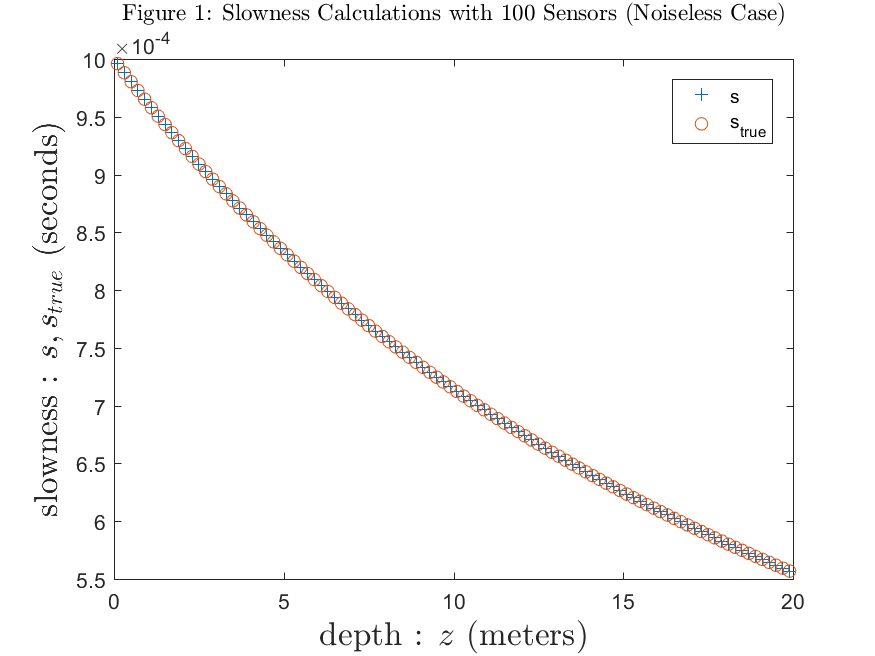
\includegraphics{Fig1.png}
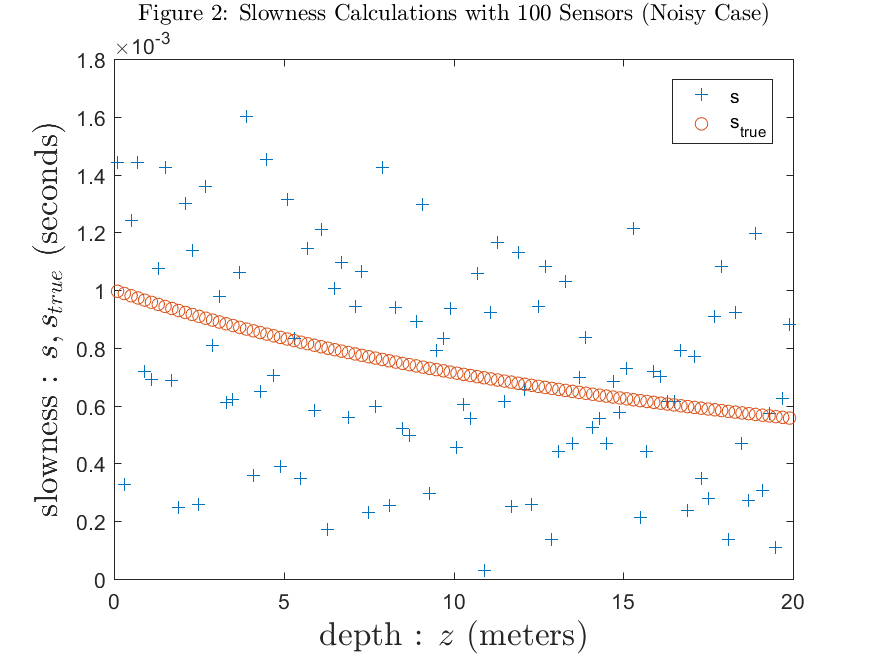
\includegraphics{Fig2.png}
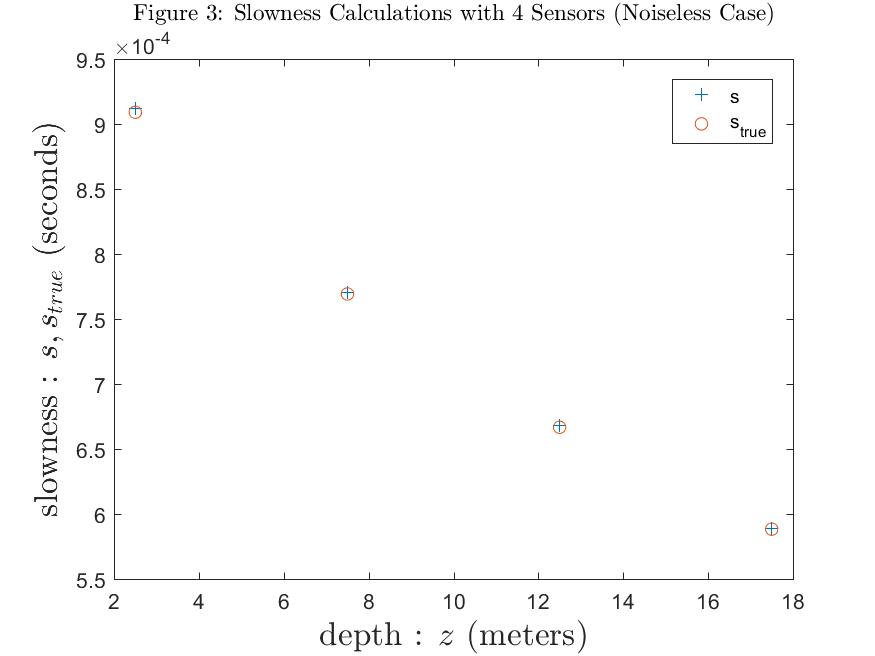
\includegraphics{Fig3.png}
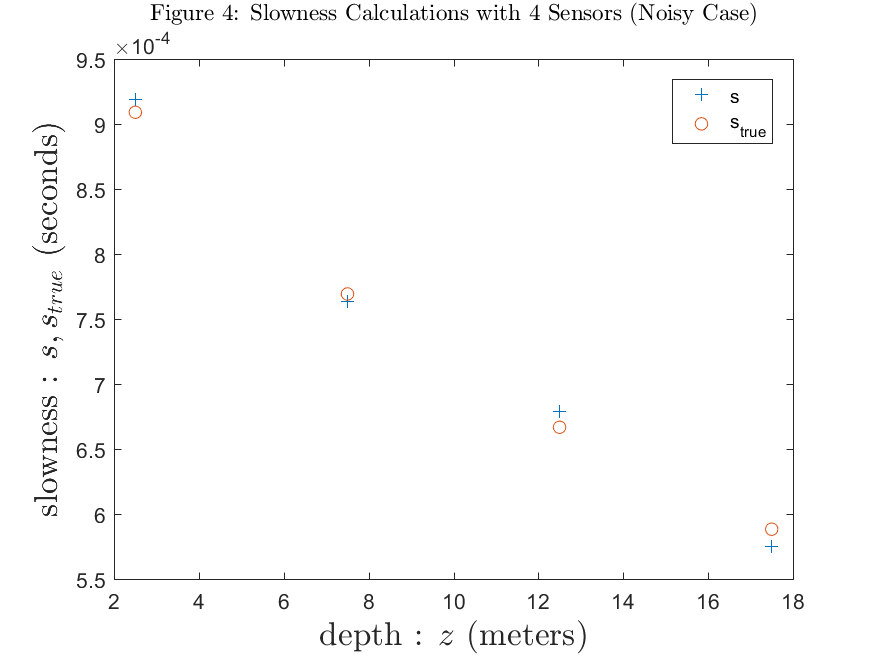
\includegraphics{Fig4.png}

\end{document}